\documentclass[letterpaper]{article}

\usepackage{aaai}
\usepackage{times}
\usepackage{helvet}
\usepackage{courier}
\usepackage{tikz}
\usetikzlibrary{arrows.meta, positioning}
\usepackage{courier}
\frenchspacing

\usepackage{amsthm}
\newtheorem{assumption}{Assumption}
\newtheorem{remark}{Remark}
\newtheorem{proposition}{Proposition}
\newtheorem{theorem}{Theorem}
 
\usepackage{amsmath, amssymb, bm}
\usepackage{booktabs}
\usepackage{etoolbox}
\usepackage[ruled,vlined,linesnumbered]{algorithm2e} 
\usepackage{xcolor}
\usepackage{comment}
\usepackage{tikz}
\usetikzlibrary{positioning, fit, backgrounds}
% Do NOT use geometry with aaai two-column style.
% \usepackage[margin=1in]{geometry}

% Make displayed equations smaller.
\AtBeginEnvironment{equation}{\small}
\AtBeginEnvironment{align}{\small}
\AtBeginEnvironment{align*}{\small}

% Compact displayed equations.
\setlength{\abovedisplayskip}{4pt}
\setlength{\belowdisplayskip}{4pt}
\setlength{\abovedisplayshortskip}{3pt}
\setlength{\belowdisplayshortskip}{3pt}

% Compact tables.
\newcommand{\tablesize}{\small}

\pdfinfo{
/Title (Two-Layer MILP Formulation for Multi-Building Energy Management)
/Author ()
}

\setcounter{secnumdepth}{0}

% ===================================================================
% Notation macros: change once, propagate everywhere.
% Indexed families take arguments, e.g. \soc{t}{v} -> \soc{t}{v}.
% ===================================================================
% --- Sets, indices, time
\newcommand{\Dset}{\mathcal{D}}              % days in billing cycle
\newcommand{\Tset}{\mathcal{T}}              % all time steps
\newcommand{\Td}{\mathcal{T}_{d}}              % steps of day d
\newcommand{\Tdv}{\mathcal{T}_{d}^{v}}           % steps of v's session on day d
\newcommand{\Vset}{\mathcal{V}}              % persistent users
\newcommand{\Vd}[1]{\mathcal{V}_{#1}}          % users with a session on day #1
\newcommand{\Kv}{\mathcal{K}_{v}}              % sessions of user v
\newcommand{\Tvk}{\mathcal{T}_{v,k}}           % steps of session k of user v
\newcommand{\dt}{\Delta t}                   % step length (h)
\newcommand{\evwin}[1]{\mathcal{T}^{\mathrm{DR}}_{#1}}         % DR event window of day #1
\newcommand{\tarr}{t_{\mathrm{arr}}}
\newcommand{\tdep}{t_{\mathrm{dep}}}
\newcommand{\treq}{t_{\mathrm{req}}}
% --- EVs, SoC, persistence
\newcommand{\soc}[2]{E_{#1}(#2)}             % SoC of #2 at time #1
\newcommand{\Earr}{E_{\mathrm{arr}}}
\newcommand{\Edep}{E_{\mathrm{dep}}}
\newcommand{\Ereq}{E_{\mathrm{req}}}
\newcommand{\Eneg}{E_{\mathrm{neg}}}
\newcommand{\Emin}{E_{\mathrm{min}}}
\newcommand{\Emax}{E_{\mathrm{max}}}
\newcommand{\wext}{w^{\mathrm{ext}}}          % external charging price
\newcommand{\Tpeak}{\mathcal{T}^{\mathrm{peak}}}
\newcommand{\pmax}{p^{\max}}
\newcommand{\pmaxpast}{p^{\max}_{\mathrm{past}}}
\newcommand{\assign}{\phi}                    % EV-to-charger assignment map
\newcommand{\pidr}{\pi^{\mathrm{DR}}}
\newcommand{\pich}{\pi^{\mathrm{ch}}}
\newcommand{\pineg}{\pi^{\mathrm{neg}}}
\newcommand{\Uflex}{U^{\mathrm{flex}}}
\newcommand{\Ubuf}{U^{\mathrm{buf}}}
\newcommand{\psihat}{\hat{\psi}}
\newcommand{\Pmaxhat}{\hat{P}_{\max}}
\newcommand{\Omeps}{\Omega_{\varepsilon}}
\newcommand{\Eext}{E_{\mathrm{ext}}}        % off-site (external) energy use
\newcommand{\banked}[2]{X(#1,#2)}            % banked excess at departure
\newcommand{\survived}[2]{S(#1,#2)}          % survived excess at arrival
\newcommand{\yieldf}[2]{\rho(#1,#2)}         % per-user yield
\newcommand{\accept}[2]{o(#1,#2)}            % over-charge acceptance
\newcommand{\buff}[1]{B_{#1}}                % realizable buffer of day #1
\newcommand{\buffhat}[1]{\hat{B}_{#1}}       % its day-ahead forecast
\newcommand{\ohat}{\hat{o}}                  % acceptance estimate
\newcommand{\rhohat}{\hat{\rho}}             % yield estimate
% --- Chargers, load, tariffs
\newcommand{\Nc}{N_{c}}
\newcommand{\rate}[2]{r_{#1}^{#2}}           % charging rate of #2 at #1
\newcommand{\rmin}[1]{r_{\min}^{#1}}
\newcommand{\rmax}[1]{r_{\max}^{#1}}
\newcommand{\avail}[2]{a_{#1}^{#2}}          % availability indicator
\newcommand{\Ptot}[1]{P_{#1}}                % total power draw
\newcommand{\bload}[1]{b_{#1}}               % non-EV building load
\newcommand{\we}[1]{w_{#1}^{e}}              % TOU energy price
\newcommand{\wdr}{w^{d}}                      % demand rate
\newcommand{\Kbatt}{K_{\mathrm{batt}}}
\newcommand{\Ksoc}{K_{\mathrm{SOC}}}
% --- Demand response
\newcommand{\FSL}{\mathrm{FSL}}
\newcommand{\Phist}{P^{\mathrm{hist}}}
\newcommand{\winc}{w^{\mathrm{inc}}}            % per-day capacity rate (tariff family w)
\newcommand{\Kfsl}{K_{\mathrm{FSL}}}
\newcommand{\vio}[1]{\sigma_{#1}}            % FSL violation slack
\newcommand{\Cinc}[1]{C_{#1}^{\mathrm{inc}}} % capacity payment
\newcommand{\Cpen}[1]{C_{#1}^{\mathrm{pen}}} % violation penalty
% --- Negotiation, payments, decisions
\newcommand{\Umu}[1]{U(#1)}                  % marginal utility [CONSENT]
\newcommand{\gch}[2]{g_{#1}^{#2}}            % energy charged
\newcommand{\ucost}[2]{\zeta_{#1}^{#2}}      % user daily cost
\newcommand{\zund}[2]{z_{#1}^{#2}}           % unmet floor energy
\newcommand{\qdis}[2]{q_{#1}^{#2}}           % discharged energy
\newcommand{\act}[1]{A_{#1}}                 % charging action
 
\title{P-CONSENT}

\author{}
\date{}

\begin{document}

\maketitle

%==============================================================
% \section{Introduction} 

For commercial buildings, electricity costs are determined not only by total energy consumption but also by peak power: the demand charge, levied on the single highest power draw of a billing cycle, can account for over 30\% of the total bill \cite{neufeld1987demandcharge,neubauer2014demandcharge}.In addition, utilities operate demand response (DR) programs that provide a recurring capacity incentive to buildings that commit to a Firm Service Level (FSL), a limit on the power draw during grid stress events, and that impose penalties when the cap is violated during a called event~\cite{}. Traditionally, building operators curtail their electricity usage and physically turn off appliances to meet these curtailments~\cite{} which can cause inconvenience to the employees. In this work, we propose another avenue to achieve curtailment by leveraging the employee-owned electric vehicles (EVs) and charging facilities that commercial buildings typically have, incentivizing their use for building load management, while allowing users autonomy to refuse charging at the building. The growing presence of EVs at workplace facilities, along with bidirectional charging, is a resource suited to both objectives: a fleet of behind-the-meter batteries that can charge during low-price periods and discharge during peaks, reshaping the building's net load without curtailing building services~\cite{}. We show that by strategically negotiating with privately owned employee EVs having predictable, regular charging schedules at the building, a building operator can achieve lower monthly peaks (lower demand charges) and increase the FSL curtailment value, thereby increasing DR incentives and further reducing the building's electricity cost. The negotiations are targeted toward trading off a user's flexibility in state of charge (SoC) requirements and departure delays for monetary benefits.

Curtailment using the EVs, however, exposes a structural asymmetry between the building operator and the users. The capacity payment is earned by committing, a day or more in advance, to deliver load reduction during events whose timing the building does not control. Unlike a stationary battery, the EVs that help fulfil this commitment are intermittently available, since EVs arrive and depart according to their users' schedules, and are self-consuming. The energy stored in a vehicle may be expended in subsequent travel, with availability determined by charging decisions made on the preceding days \cite{iccps2026_pv2b}. Moreover, the EVs are owned by users who are self-interested and need to be well compensated for helping the building lower its bill. A building that commits to a lower, more aggressive FSL earns greater capacity revenue but bears the full delivery risk, and it needs to strategize and anticipate the user's behavior.
 
Resolving this asymmetry requires navigating a set of deeply interconnected challenges. First, the commitment is made under forecast uncertainty. The FSL must be committed before building loads, EV arrivals, and, critically, user cooperation for the day in question are realized, so the commitment is made against a forecast distribution rather than a realized schedule.  Second, the system must achieve incentive alignment without perfect user-side knowledge. Users must be compensated for flexibility in departure time and required SoC, and must not be able to profit by misreporting \cite{sen2026negotiations}. This is without any prior information available to the building about a user's preferences or a complete prediction of that user's behavior. Crucially, their negotiated SoC requirements must be met by departure. This leads to the third challenge of charging decisions. The charging actions need to balance the power use in high and low load times of the day. Moreover, the charge in EVs is temporally coupled. The energy buffer available for discharge on a high peak or a DR event day is the outcome of past charging decisions, off-site usage of the EVs, and the recurrence pattern of the EV. \cite{iccps2026_pv2b}. Single-day formulations, widely used in the EV charging literature, do not account for the temporal coupling across days, and the demand charge based on the monthly peak power defines sparse and delayed rewards.
 
Prior work addresses these challenges in isolation \textcolor{red}{(related-work section pending)}. Two-stage DR mechanism design \cite{satchidanandan2022two} formalizes the day-ahead-commitment, real-time-delivery structure, but for resources that are dispatchable and stationary rather than intermittently available, have private information, and are self-consuming. Strategy-proof daily negotiation \cite{sen2026negotiations} prices user flexibility and guarantees incentive compatibility, but it does not have temporal coupling across days, so that stored energy cannot be carried across day boundaries and the discharge depth available on a peak day is limited to the incidental surplus with which users arrive. Real-time V2B charging control with user persistence \cite{iccps2026_pv2b} handles the inter-day EV arrivals and charge planning, but it presumes complete cooperation from EV users and does not provide a structure for incentivizing. The reward is only for the long-horizon, sparse demand charge.  None of these approaches individually enables a building operator to provide a prior FSL commitment while requiring no prior commitment from its users.
 
We close this gap with P-CONSENT, a three-layer architecture with a deliberately asymmetric commitment structure. 
Layer~1, a day-ahead optimization between the building and the grid, determines the committed FSL. The commitment and its associated penalty are borne exclusively by the building. However, as shown later, the system tries to reduce the penalties by incorporating them in user negotiations. 
Layer~2, a negotiation mechanism using Monte-Carlo sampled model predictive control (MC-MPC), generates daily user options consistent with the previously fixed FSL. The layer compensates users for realized peak shaving and FSL penalty avoidance, with battery degradation incorporated into the payment. Users are negotiated with only at each arrival, with no future commitments required. 
Layer~3, another real-time Monte Carlo model predictive controller (MC-MPC) \cite{iccps2026_pv2b}, delivers against the committed FSL and the negotiated user requirements at minimum cost, using future samples and re-optimizing at fixed intervals, using updated building loads and EV status. On off-peak days, the controller over-charges consenting users above their negotiated SoC requirements, and is carried over to the subsequent day \cite{iccps2026_pv2b}. On high-peak or DR event days, it discharges the accumulated excess, along with smart planning for intra-day charge/discharge decisions.
Across the system, information flows unidirectionally, from the FSL commitment to the negotiation mechanism to the charging controller.
Our contributions are: 

\begin{itemize} 

\item \textbf{A formulation for DR participation backed by an intermittently available, self-consuming, temporally coupled resource (EVs) with private information}, with a three-layer decision structure whose within-day information flow is unidirectional (from the FSL commitment to the negotiation mechanism to the charging controller) and whose cross-day loop closes through the persistent SoC buffer.
% (Section~\ref{sec:formulation}). 

% \item \textbf{A characterization of the feasible commitment set}, establishing that the set of FSLs deliverable at a given risk level grows monotonically with the forecast buffer, thereby formalizing the manner in which persistence-aware over-charging expands upstream commitment capacity (Proposition~\ref{prop:monotone}), together with a commitment-depth parameter that prices the building's delivery risk and a newsvendor-type characterization of the risk-neutral optimal commitment, which anchors the depth parameter to a principled operating point. 

\item \textbf{A rigorous user negotiation mechanism} where user offers are weakly strategy-proof, incentive compatible and allow voluntary participation.
% we state precisely which of CONSENT's guarantees transfer unchanged and which require restatement under the over-charge policy (Section~4). 

\item \textbf{An evaluation on real building, tariff, and EV fleet data} from a commercial facility (Nissan Advanced Technology Center, Silicon Valley), demonstrating that the combined architecture weakly dominates building-only, negotiation-only, and persistence-only baselines with respect to both building and user cost, with sensitivity analyses over the cost-sharing parameter $\alpha$ \cite{sen2026negotiations} and the commitment depth (Section~\ref{sec:eval}). 

\end{itemize}

% \section{Problem Formulation}\label{sec:formulation}

% Three-policy-lane view of P-CONSENT. The three policies are the primary
% structure: pi^DR (day-ahead), pi^ch (every dt), pi^neg (per arrival), each
% on its own clock. Vertical arrows are the within-day dependency (FSL ->
% charging feasible set -> negotiation options); the dashed arrow is the sole
% cross-day link (surviving buffer). Not a timeline: see Sec. 4.
% Requires \usetikzlibrary{positioning, fit, backgrounds, arrows.meta}.
\begin{figure*}[t]
\centering
\newcommand{\ltitle}{\bfseries}%
\newcommand{\leqn}{\scriptsize\itshape\color{black!55}}%
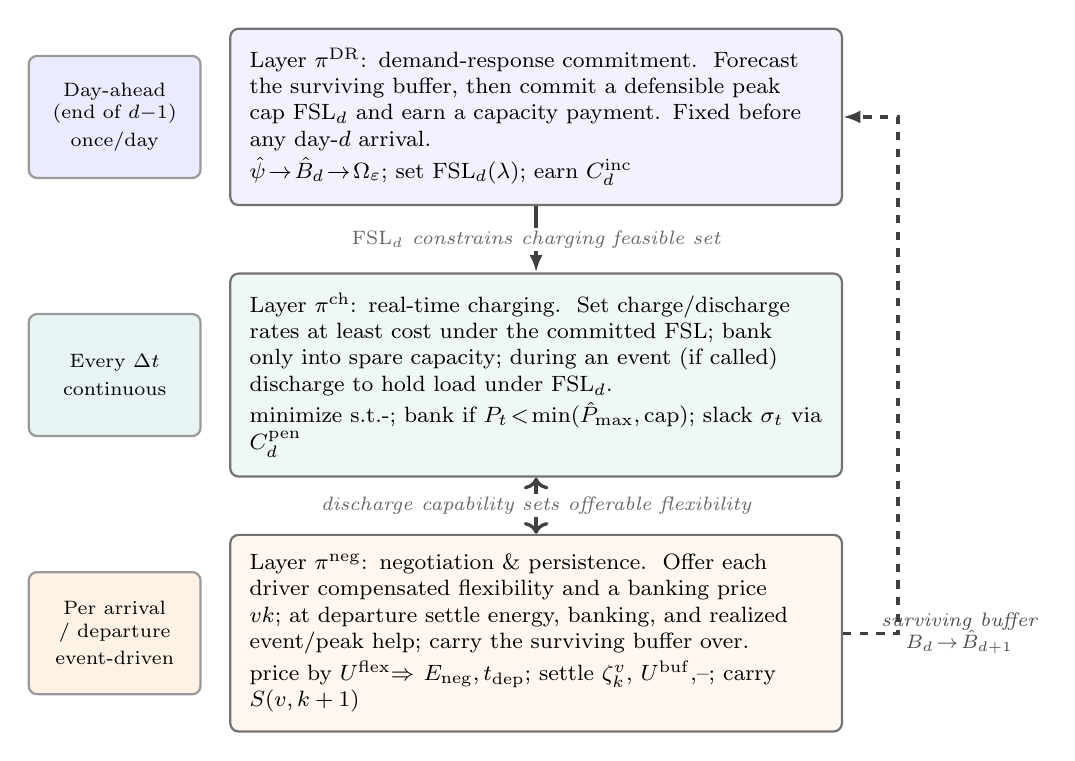
\begin{tikzpicture}[
  font=\footnotesize,
  every node/.style={transform shape},
  lane/.style={rectangle, rounded corners=3pt, draw=black!55, thick,
               align=left, inner sep=7pt, text width=0.60\textwidth,
               minimum height=1.55cm},
  clock/.style={rectangle, rounded corners=3pt, draw=black!40, thick,
                fill=white, align=center, inner sep=4pt, text width=1.9cm,
                minimum height=1.55cm, font=\scriptsize},
  dep/.style={-{Latex[length=2.2mm]}, very thick, black!75},
  back/.style={-{Latex[length=2.2mm]}, very thick, dashed, black!75},
  deplab/.style={font=\scriptsize\itshape, text=black!60, align=center, fill=white, inner sep=1pt}
]
% ============ LANE 1: pi^DR (day-ahead) ============
\node[clock, fill=blue!8] (cDR) {\ltitle Day-ahead\\(end of $d{-}1$)\\[2pt]\leqn once/day};
\node[lane, fill=blue!5, right=0.35cm of cDR] (DR) {%
{\ltitle Layer $\pidr$: demand-response commitment.}\ \ Forecast the surviving
buffer, then commit a defensible peak cap $\FSL_d$ and earn a capacity payment.
Fixed before any day-$d$ arrival.\\[2pt]
{\leqn $\psihat\!\to\!\buffhat{d}\!\to\!\Omeps$; set
$\FSL_d(\lambda)$;\ earn $\Cinc{d}$}};

% ============ LANE 2: pi^ch (every dt) ============
\node[clock, fill=teal!9, below=1.7cm of cDR] (cCH) {\ltitle Every $\dt$\\[2pt]\leqn continuous};
\node[lane, fill=teal!6, right=0.35cm of cCH] (CH) {%
{\ltitle Layer $\pich$: real-time charging.}\ \ Set charge/discharge rates at
least cost under the committed FSL; bank only into spare capacity; during an
event (if called) discharge to hold load under $\FSL_d$.\\[2pt]
{\leqn minimize s.t.\--;
bank if $\Ptot{t}\!<\!\min(\Pmaxhat,\text{cap})$; slack $\vio{t}$ via $\Cpen{d}$}};

% ============ LANE 3: pi^neg (per arrival) ============
\node[clock, fill=orange!10, below=1.7cm of cCH] (cNEG) {\ltitle Per arrival\\/ departure\\[2pt]\leqn event-driven};
\node[lane, fill=orange!6, right=0.35cm of cNEG] (NEG) {%
{\ltitle Layer $\pineg$: negotiation \& persistence.}\ \ Offer each driver
compensated flexibility and a banking price $\pbank{v}{k}$; at departure settle
energy, banking, and realized event/peak help; carry the surviving buffer over.\\[2pt]
{\leqn price by $\Uflex$$\Rightarrow\!\Eneg,\tdep$; settle
$\ucost{k}{v}$, $\Ubuf,\Udc$--;
carry $\survived{v}{k+1}$}};

% ============ WITHIN-DAY DEPENDENCY (top -> down) ============
\draw[dep] (DR.south) -- (CH.north)
  node[deplab, midway] {$\FSL_d$ constrains charging feasible set};
\draw[dep, <->] (CH.south) -- (NEG.north)
  node[deplab, midway] {discharge capability sets offerable flexibility};

% ============ CROSS-DAY LINK (bottom -> up, dashed) ============
\draw[back] (NEG.east) -- ++(0.7,0)
  node[midway, right, font=\scriptsize\itshape, text=black!70, align=center]
    {surviving buffer\\ $\buff{d}\!\to\!\buffhat{d+1}$}
  |- (DR.east);

  

\end{tikzpicture}
\caption{The three policies of P-CONSENT, each acting on its own clock:
$\pidr$ commits the firm service level a day ahead, $\pich$ sets charging and
discharging rates every $\dt$, and $\pineg$ negotiates flexibility and settles
payments at each arrival and departure. Solid vertical arrows are the sole
within-day dependency, the committed FSL constrains the charging feasible set,
which in turn sets the flexibility the negotiation can offer; this is a
dependency, not a temporal order, since the charging and negotiation epochs
interleave continuously through the day (the problem definition (Section~\ref{sec:formulation})). The dashed
arrow is the only coupling between days: the buffer that survives a driver's
trip becomes tomorrow's deliverable buffer and sharpens the forecast that sets
the next commitment.}
\label{fig:processflow}
\end{figure*}


We consider a single commercial building that manages its own EV charging infrastructure, serves a population of persistent EV users, and participates in a utility demand response (DR) program. Three decisions act on the system at three timescales (Figure~\ref{fig:processflow}): a day-ahead \emph{commitment} of a Firm Service Level to the utility (policy $\pidr$), real-time \emph{charging} and discharging (policy $\pich$), and per-arrival \emph{negotiation} of compensated adjustments to a user's required SoC and departure time (policy $\pineg$). We first declare the shared physical layer (Section~\ref{sec:specs}), then define each of the three sub-problems, their decisions, constraints, and objective contribution. 
% Section~\ref{sec:coupled} then assembles them into the single sequential problem they jointly approximate and states its ideal solution. 
The complete variable dependency structure is summarized in Table~\ref{tab:vartree}.








\subsection{Specifications}\label{sec:specs}

\paragraph{Time structure.} The billing cycle consists of days $d \in \Dset$. Each day is discretized into time steps $t \in \Td$ of length $\dt$ (e.g., 15 minutes), and $\Tset = \cup_d \Td$. The demand charge is assessed over designated peak periods $\Tpeak \subseteq \Tset$. Control decisions are taken at the start of each step and held constant for its duration.

\paragraph{Persistent users and sessions.} Let $\Vset$ be the set of EV
users, each with a consistent identity across the billing cycle. User $v$'s visits are indexed by sessions $k \in \Kv$, with first session $k = 0$; session $k$ spans $[\tarr(v,k), \tdep(v,k)] \subseteq \Tset$, and $\Tvk$ denotes its time steps. Sessions need not occur on consecutive days; the formulation accommodates arbitrary gaps between visits. At plug-in, the arrival time $\tarr(v,k)$ and arrival SoC $\Earr(v,k)$ are observed, and the user reports a required departure SoC $\Ereq(v,k)$ and departure time $\treq(v,k)$. Let $\Vd{d} \subseteq \Vset$ denote the users with a session active on day $d$. Per-user, per-session quantities are written $X(v,k)$ (and $X(v)$ when they depend on the user alone); within a report or agreement tuple that concerns a single fixed user-session, we drop the arguments and write, for instance, $(\Ereq, \treq)$ for brevity.

\paragraph{Battery state and persistence.} The SoC of EV $v$ at time $t$
is $\soc{t}{v}$, expressed in energy units (kWh) and bounded by the usable battery window:
\begin{equation}\label{eq:socbounds}
\Emin(v) \;\le\; \soc{t}{v} \;\le\; \Emax(v).
\end{equation}
Within a session, the SoC evolves as
\begin{equation}\label{eq:soc}
\soc{t+1}{v} \;=\; \soc{t}{v} + \rate{t}{v}\,\dt,
\end{equation}
where $\rate{t}{v}$ (kW) is the charging rate, negative for discharge; since at most one session is active at any time, the session index is omitted from per-step quantities. The EV user arrives with a SoC requirement for the session $\Ereq(v,k)$ (kWh). As part of negotiations, the users can accept a different negotiated SoC $\Eneg(v,k)$. This is separate from the SoC at departure $\Edep(v,k)$ (kWh). Between sessions $k$ and $k{+}1$, the EV consumes $\Eext(v,k)$ energy off-site (kWh), net of any external charging, with $\Eext(v,k) \le \Edep(v,k)$. Combined, 
\begin{equation}\label{eq:carryover}
\Earr(v,k{+}1) \;=\; \Edep(v,k) - \Eext(v,k),
\end{equation}
where $\Edep(v,k)$ is the SoC at departure from session $k$. The arrival SoC is therefore exogenous only at $k = 0$; for every later session it is determined by \eqref{eq:carryover}, which is precisely what makes the fleet an inter-temporally coupled resource and what single-day formulations cannot represent. 

\begin{assumption}[Exogenous off-site usage]\label{as:exo}
$\Eext(v,k)$ is unaffected by the over-charge decision; cost-free energy does not induce additional vehicle usage. This is a behavioral assumption subject to a potential rebound effect, revisited when interpreting the measured yield (Section~\ref{sec:eval}).
\end{assumption}


\paragraph{Chargers and assignment.} The building operates a set
$\mathcal{C}$ of heterogeneous charger types with $N_c$ units of type $c$, rate limits $[\rmin{c}, \rmax{c}]$ ($\rmin{c} < 0$ only for bidirectional chargers). Charging is modeled as lossless; discharge delivers energy to the building at round-trip efficiency $\eta \in (0,1]$, so that banked excess of $E$ kWh yields $\eta E$ kWh at the meter. An assignment map $\assign_t : \mathcal{V}_t \leftrightarrow \mathcal{C}_t$ matches present EVs to chargers one-to-one, first-come, first-served, fixed for the duration of the session; an EV that arrives when no charger is free cannot participate. The availability indicator is $\avail{t}{v} \in \{0,1\}$. Charging-rate slowdown at high SoC is modeled by piecewise-linear segments and deferred to the appendix.




\paragraph{Building power and electricity cost.} The building's total
power draw is
\begin{equation}\label{eq:load}
\Ptot{t} \;=\; \bload{t} + \sum_{v \in \Vset} \avail{t}{v}\,\rate{t}{v},
\qquad \Ptot{t} \ge 0,
\end{equation}
where $\bload{t}$ (kW) is the non-EV building load. The energy cost at step $t$ is $\Phi^{e}_t = \we{t}\,\Ptot{t}\,\dt$ with time-of-use price $\we{t}$ (\$/kWh), and the energy cost attributed to user $v$ sums the energy $\gch{t}{v} \ge 0$ delivered to their EV; discharged energy carries no meter credit, its value reaching the user exclusively through the replay incentives of Section~\ref{sec:negotiation}. The demand cost is
\begin{equation}\label{eq:peak}
\Phi^{d} = \wdr{}\cdot \max_{t \in \Tpeak} \Ptot{t}
\end{equation}
Discharging accrues a degradation cost $\Kbatt$ per kWh of throughput, tracked by the one-sided variable $\qdis{t}{v} \ge -\rate{t}{v}\dt$ (nonzero only on discharge, where $\rate{t}{v}<0$; pinned to zero on charge by the objective), and departing below the negotiated floor incurs $\Ksoc$ per kWh of shortfall $\zund{k}{v}$. The building can build towards and forecast a realizable SoC buffer $\buffhat{d}$ for the upcoming DR day, using the EVs present in the current day and that have been present in the past.


\paragraph{Policies.} The building's policy is the triple $\pi =
(\pidr, \pich, \pineg)$ with decision epochs at the end of each day, at every time step, and at every user arrival, respectively. All derived quantities below (SoC trajectories, peaks, costs) are implicitly determined by $\pi$ and the realized user choices; we omit this dependence from the notation for readability.

% \subsection{The FSL Commitment Sub-Problem ($\Pdr$)}\label{sec:dr}

\paragraph{Demand Response Commitment.} For a DR event announced for day $d$, the peak level commitment, Firm Service Level $\FSL_d$ (kW) has to be made ahead of time on day $d{-}n$, where $n$ is the notification time from the power utility. \textcolor{red}{check} The operator is expected to have a tolerance of $\varepsilon$ towards any deviation if the committed FSL. No other decision is taken at this layer. There can be multiple DR events per month, and each has its own commitment and penalties.

\paragraph{Payment and penalty.} The utility registers a baseline
$\Phist$ (kW) at enrollment from historical billing data. The capacity payment and the violation penalty are
\begin{equation}\label{eq:dr}
\Cinc{d} = \winc\,(\Phist - \FSL_d), \qquad
\end{equation}
\begin{equation}
\Cpen{d} = \Kfsl \sum_{t \in \evwin{d}} (P_{t} - \FSL_d) \Delta t \le \sigma^i_t\ 
% ; \quad \forall t \in {\evwin{d}}
%  = \Kfsl \sum_{t \in \evwin{d}} \vio{t}\,\dt,
\end{equation}
where $\winc$ (\$/kW) is the per-day-normalized capacity rate and $\vio{t} = \max(0,\, \Ptot{t} - \FSL_d)$ is the FSL violation, i.e., sum of energy (kWh) used above the FSL during the DR event $\evwin{d}$. The event window $\evwin{d}$ and the demand-charge peak period $\Tpeak$ are distinct time sets and need not coincide.

\begin{remark}[DR Program choice]\label{rem:program}
Deployed programs differ in commitment cadence: the Base Interruptible Program fixes the FSL at enrollment for a season, whereas capacity bidding programs admit nomination with day-ahead and day-of options. We model a day-ahead re-committable FSL, corresponding most closely to the day-ahead capacity-bidding option, and normalize the capacity rate to $\winc$ per committed day. An enrollment-fixed FSL is the constrained special case $\FSL_d \equiv \FSL$ and is reported in the sensitivity analysis.
\end{remark}


\paragraph{User Cost, Choices and options.} User $v$'s choice $\theta_v \in \boldsymbol{\theta}$ records the observed arrival data and the negotiated departure SoC and time. Users are requested to be flexible in their requests and are parameterized by levels $l \in \{0, \ldots, L\}$ with deviation bounds $\Delta e^{\max}_l$ and $\Delta t^{\max}_{\mathrm{dep},l}$; level $l = 0$ is the user's exact request, together with a reject-all choice priced at the external rate $\wext$. Each user has to pay a charging cost $\zeta_v$ depending on the option they choose. 

% \paragraph{Over-charge offer, and the banking price.}
% Independently of the chosen level, the user may consent to over-charge above the negotiated floor, recorded by $\accept{v}{k} \in \{0,1\}$. Consenting is the user's only SoC banking decision, with the amount and timing being controlled by the operator (building), which removes any reportable banking quantity from the user's strategy space. The departing SoC excess $\banked{v}{k}$ is priced at the banking rate
% \begin{equation}\label{eq:pbank}
% \pbank{v}{k} \;=\;  
% \begin{cases}  
% {w}^{e}_{k}, & \text{if DR event not announced} \\  
% 0, & \text{if DR event is announced}  
% \end{cases} 
% \end{equation}
% where ${w}^{e}_{k}$ is the energy price paid.

\paragraph{Total Cost.}  
The building’s total cost is over a monthly billing period under demand response, negotiation, and charging policies, and the user choices. For convenience, we omit explicit notation of this dependence, writing the cost function as
\begin{equation}\label{eq:obj}
% \small
\begin{split}
& J = \sum_{t \in \mathcal{T}} \Phi^{e}_t + \Phi^d
+ K_{\mathbf{SOC}} \sum_{v \in \mathcal{V}} \left(e^v_{\mathrm{req}} - e^v_{\mathrm{dep}} \right)\\
& + K_{\mathbf{batt}} \sum_{v \in \mathcal{V}} \sum_{t \in \mathcal{T}^v} q_t^v + \sum_{d \in \mathcal D} \Cpen{d} - \Cinc{d} 
\end{split}
\end{equation}

subject to the constraints \eqref{eq:socbounds}--\eqref{eq:dr}.



% % \section{Approach}\label{sec:approach}

% Timeline of decisions across a pre-event day and an event day, one swimlane
% per controller. Complements Fig. 1 (dependency map): this figure shows WHEN
% each policy acts and WHICH decision it takes. Lanes are independent clocks;
% arrival and control epochs interleave (no fixed order).
% Requires \usetikzlibrary{arrows.meta, positioning, backgrounds}.
\begin{figure*}[t]
\centering
\begin{tikzpicture}[
  font=\scriptsize,
  lanelab/.style={align=center, anchor=east, font=\scriptsize},
  evt/.style={font=\tiny\itshape, text=black!65, align=center},
  arr/.style={-{Latex[length=1.6mm]}, thick},
  x=1cm, y=1cm
]
% day d-1: x in [0,6.4]; overnight: [6.4,8.0]; day d: [8.0,14.4]
% lanes: DR y=2.5, ch y=1.25, neg y=0
% ---------- event window band (day d, behind everything) ----------
\begin{scope}[on background layer]
\fill[red!8] (11.4,-0.75) rectangle (13.3,3.05);
\draw[red!40, thin] (11.4,-0.75) rectangle (13.3,3.05);
\end{scope}
\node[evt, text=red!60!black] at (12.35,3.25) {event window $\evwin{d}$ (4--5\,h)};
% ---------- day headers ----------
\node[font=\scriptsize\bfseries] at (3.2,3.6) {day $d{-}1$ (pre-event)};
\node[font=\scriptsize\bfseries, text=black!55] at (7.2,3.6) {overnight};
\node[font=\scriptsize\bfseries] at (9.9,3.6) {day $d$ (event called)};
\draw[black!30, thin] (0,3.4) -- (6.4,3.4);
\draw[black!30, thin, dashed] (6.4,3.4) -- (8.0,3.4);
\draw[black!30, thin] (8.0,3.4) -- (14.4,3.4);
% ---------- lane baselines ----------
\draw[blue!35, thick] (0,2.5) -- (6.4,2.5);
\draw[blue!35, thick, densely dotted] (6.4,2.5) -- (8.0,2.5);
\draw[blue!35, thick] (8.0,2.5) -- (14.4,2.5);
\draw[teal!45, thick] (0,1.25) -- (6.4,1.25);
\draw[teal!45, thick, densely dotted] (6.4,1.25) -- (8.0,1.25);
\draw[teal!45, thick] (8.0,1.25) -- (14.4,1.25);
\draw[orange!55, thick] (0,0) -- (6.4,0);
\draw[orange!55, thick, densely dotted] (6.4,0) -- (8.0,0);
\draw[orange!55, thick] (8.0,0) -- (14.4,0);
% ---------- lane labels ----------
\node[lanelab, text=blue!50!black]  at (-0.25,2.5)
  {$\pidr$ \\ {\tiny once per day}};
\node[lanelab, text=teal!50!black]  at (-0.25,1.25)
  {$\pich$ \\ {\tiny every $\dt$}};
\node[lanelab, text=orange!60!black] at (-0.25,0)
  {$\pineg$ \\ {\tiny per arrival,} \\ {\tiny departure}};
% ---------- pi^DR: start-of-day commitments ----------
\node[diamond, fill=blue!25, draw=blue!60, inner sep=1.6pt] at (0,2.5) {};
\node[evt, anchor=south west, text width=3.2cm] at (-0.05,2.64)
  {commit $\FSL_d$ for day $d$ (Alg.~\ref{alg:dr})};
\draw[arr, blue!55] (0.15,2.42) -- (0.85,1.40)
  node[evt, pos=0.75, right=1pt, text width=1.6cm] {targets steer current SoC banking};
\node[diamond, fill=blue!25, draw=blue!60, inner sep=1.6pt] at (8.0,2.5) {};
\node[evt, anchor=south west, text width=1.9cm] at (7.95,2.64)
  {commit $\FSL_{d+1}$};
\draw[arr, blue!55] (8.6,2.42) -- (8.6,1.40)
  node[evt, pos=0.45, right=1pt, text width=1.5cm] {$\FSL_d$ in effect for day $d$};
% ---------- pi^ch: control comb ----------
\foreach \xx in {0.0,0.32,...,6.4}  \draw[teal!60] (\xx,1.18) -- (\xx,1.32);
\foreach \xx in {8.0,8.32,...,14.4} \draw[teal!60] (\xx,1.18) -- (\xx,1.32);
\node[evt, anchor=north, text width=3.6cm] at (3.0,1.11)
  {Charge excess SoC when ($\Ptot{t}<\Pmaxhat$), pulled to targets (Alg.~\ref{alg:ch})};
\node[evt, anchor=north, text width=2.2cm] at (12.35,1.11)
  {discharge buffer; hold $\Ptot{t}\le\FSL_d$};
% ---------- pi^neg: arrivals and departures ----------
\foreach \xx in {1.1,1.7,2.4}
  \draw[arr, orange!75!black] (\xx,0.32) -- (\xx,0.04);
\foreach \xx in {9.1,9.7,10.4}
  \draw[arr, orange!75!black] (\xx,0.32) -- (\xx,0.04);
\foreach \xx in {4.9,5.5,6.1}
  \draw[arr, orange!75!black] (\xx,-0.04) -- (\xx,-0.32);
\foreach \xx in {13.5,13.9,14.3}
  \draw[arr, orange!75!black] (\xx,-0.04) -- (\xx,-0.32);
\node[evt, anchor=north, text width=3.2cm] at (1.75,-0.42)
  {arrivals: flexibility menu, banking consent at $\pbank{v}{k}$};
\node[evt, anchor=north, text width=3.1cm] at (5.5,-0.42)
  {departures};
\node[evt, anchor=north, text width=3.0cm] at (13.4,-0.85)
  {departures $\Ubuf$, $\Udc$};
% ---------- overnight carryover ----------
\draw[arr, black!60, densely dashed] (6.5,0.62) -- (7.9,0.62);
\node[evt, text width=1.7cm] at (7.2,1.12)
  {Excess SoC carryover};
\end{tikzpicture}
\caption{When each decision is taken, and by which controller, across a
pre-event day and an event day. The commitment policy $\pidr$ acts once per
day, at the start of the day: at the start of day $d{-}1$ it commits
$\FSL_d$ for the following day, before any day-$(d{-}1)$ or day-$d$ vehicle
has arrived, and sets the terminal targets that steer the current day's
banking. The charging policy $\pich$ acts every control step: on the
pre-event day it banks excess SoC into headroom, and inside the called
window it discharges the surviving buffer to hold the committed level. The
negotiation policy $\pineg$ acts at each arrival (flexibility menu and
banking consent) and each departure (settlement on realized quantities; on
event days, the replay shares $\Ubuf$ and $\Udc$). The three rows are
independent clocks whose epochs interleave; the commitment is fixed a full
day before the day it governs (Section~\ref{sec:coupled}).}
\label{fig:timeline}
\end{figure*}

% Section~\ref{sec:formulation} posed three sub-problems and Section~\ref{sec:coupled} showed they compose into one semi-Markov program. This section describes how each policy is computed and how the three exchange information at run time. 





\subsection{Day-Ahead Commitment ($\pidr$)}\label{sec:approach-dr}



The FSL commitment policy chooses $\FSL_d$ at the start of day $d{-}n$ by solving a day-ahead problem while evaluating its risk. It solves a MILP that minimizes expected cost over sampled days drawn from the forecast $\psihat$, providing a possible event-window peak. 
% This is the Sample Average Approximation (SAA) over the sampled future states. where the true violation probability is replaced by its empirical frequency over the sampled days. The forecast $\psihat$ already includes the SoC banking and flexibility the building anticipates, enabling the nomination to reflect the resources it expects to have. The negotiation of Section~\ref{sec:approach-neg} then realizes that flexibility on the day and settles it as revenue and user savings, but it never revises the committed level.

\begin{algorithm}[t]
\caption{$\pidr$: day-ahead commitment by scenario MILP}
\label{alg:dr}
\DontPrintSemicolon
\SetCommentSty{algocmt}
\KwIn{forecast $\psihat$ (including anticipated banking and flexibility);
event window $\evwin{d}$; delivery risk level $\varepsilon$; commitment
depth $\lambda \in [0,1]$; sample count $N$; baseline peak $\Phist$;
per-vehicle usable maxima $\{E_{\max}(v)\}$}
\KwOut{committed level $\FSL_d$}
set $\etarget{v}{k} \leftarrow E_{\max}(v)$ for every user $v$ and session $k$
\tcp*{uniform \emph{aspiration}; clipped by the headroom gate in $\pich$}
Draw $N$ sampled days $\omega_1,\dots,\omega_N \sim \psihat$ (arrivals,
required SoC, off-site use)\;
solve the day-ahead scenario MILP once over $\omega_1,\dots,\omega_N$,
minimizing expected cost \tcp*{risk-neutral nomination}
\lFor{each $\omega_i$}{$m_i \leftarrow \max_{t \in \evwin{d}} \Ptot{t}$
\tcp*[f]{window peak realized by that solve}}
$\min\Omeps \leftarrow$ the $(1-\varepsilon)$ empirical quantile of
$\{m_1,\dots,m_N\}$ \tcp*{deepest cap held on $\ge 1-\varepsilon$ of days}
$\FSL_d \leftarrow \Phist - \lambda\,\bigl(\Phist - \min \Omeps\bigr)$
\tcp*{commitment-depth interpolation}
\Return $\FSL_d,\ \{\etarget{v}{k}\}$\;
\end{algorithm}

% A cap $F$ is held on sampled day $i$ exactly when that day's window peak $m_i = \max_{t\in\evwin{d}} \Ptot{t}$ stays at or below it: \begin{equation}\label{eq:xflag} \text{day $i$ holds cap $F$} \;\Longleftrightarrow\; m_i \le F \;\Longleftrightarrow\; \Ptot{t} \le F \ \text{for every } t \in \evwin{d}. \end{equation} The commitment is thus evaluated \emph{jointly} over the window: a day counts as a failure if it breaches the cap at \emph{any} within-window step, not as a per-step average. A level that passes most steps can still fail the joint test, and only the joint test matches the delivery guarantee the building sells. Taking the $(1-\varepsilon)$ quantile of the peaks $\{m_i\}$ therefore returns $\min\Omeps$, the deepest cap held on at least a $1-\varepsilon$ fraction of sampled days. Because the peaks $m_i$ are read from the risk-neutral solve, which was not itself trying to reach deeper caps, $\min\Omeps$ is a \emph{conservative} estimate of the deepest deliverable level; a per-candidate delivery pass would only lower it, so the reported commitments understate rather than overstate what the fleet can hold. The interpolation returns the null commitment $\FSL_d = \Phist$ at $\lambda = 0$ and this deepest $\varepsilon$-feasible level at $\lambda = 1$, and Proposition~\ref{prop:newsvendor} identifies the risk-neutral anchor within this family. 

The terminal targets $\etarget{v}{k}$ set how much buffer the commitment layer \emph{asks} each user to leave behind; they are a soft pull, not a hard requirement. The current implementation uses a uniform aspiration, $\etarget{v}{k} = E_{\max}(v)$, nominally asking every vehicle to bank to its usable maximum. This does not mean vehicles are charged to full: the target only biases dispatch, and the banking it induces is admitted by $\pich$ only into headroom below the estimated and running peaks (Section~\ref{sec:approach-ch}) and always within the committed FSL and rate limits. A vehicle therefore reaches $E_{\max}$ only if it can do so without violating the estimated peak $\Pmaxhat$. 

% The uniform aspiration is deliberately simple and, being maximal, un-prioritized: it does not shape the buffer to the commitment's actual shortfall or choose which vehicles should carry it. A refinement that distributes only the buffer the commitment requires (from $\min\Omeps$), across users in proportion to their forecast availability, would reduce unnecessary banking and its degradation cost without changing the interface to $\pich$; we treat it as future work and report results under the uniform aspiration.

\subsection{Real-Time Charging ($\pich$)}\label{sec:approach-ch}

The charging policy is a Monte Carlo model-predictive controller (MC-MPC): it acts every control step under a receding horizon, and handles the uncertainty in future arrivals by sampling. At step $t$ it draws $K$ samples from $\psihat$, solves a mixed-integer program over the remaining horizon for each with a common first action and the committed $\FSL_d$. The first action at the current time $t$ is applied, and rolls forward. The objective is Eq.~\eqref{eq:chobj}, combining energy, demand, the FSL penalty, degradation, and the end-of-day SoC banking reward $\Kbank{v}\bshort{v}$ that pulls departures toward $\etarget{v}{k}$.


\begin{algorithm}[tbph]
\caption{P-V2B Charging Optimization}
\label{alg:MP-MPC}
\KwIn{Initial state $S_0$, number of samples $N_f$, billing period $T$, estimated monthly peak power $\hat{P}^{max}$ 

}
\KwOut{Charging decisions $A_t$}

\For{$t = 0$ \KwTo $\mathcal{T}$}{

    Check EV departures and free assigned chargers\;
    Assign chargers to new arrivals using FCFS\; 
    Observe current state $\State_t$\;
    Future trajectory set $\mathcal{F} \leftarrow \emptyset$\; 
    \For{$i = 1$ \KwTo $N_f$}{
       Sample trajectory $f$ from the generative model given $\State_t$, simulate from $t{+}1$ to $t_{eod}$, and add $f$ to $\mathcal{F}$\;
    }
    Get $A_t$ by solving optimization in Eq.~(\ref{eq:ns_objective}) 
    
    Refine action to $\tilde{A}_t=f_{\text{refine}}(A_t, \hat{P}^{\max})$ by Eq.~(\ref{eq:force_charge})  
    % Subject to: $A_t$ is shared across all $f$, and feasibility constraints (Section~\ref{sec:constraints})\;
    
    Apply $\tilde{A}_t$ and update system state to $\State_{t+1}$\;
}
% \vspace{-1mm}
\end{algorithm}

Two components govern SoC banking. The target SoC $\etarget{v}{k}$, through $\Kbank{v}\bshort{v}$, states the size of the buffer and the  estimated peak $\Pmaxhat$ and the running cycle peak $\pmaxpast$ estimated cap $\Pmaxhat$ states when accumulating it is favorable. Hence, banking never creates a new demand-charge peak. When no event is anticipated, $\muDR = 0$ and $\Kbank{v} = 0$, and the composition reduces exactly to the opportunistic headroom rule of P-V2B, which is the null-commitment special case. 


% The dual $\muDR$ on the FSL-delivery requirement is the shadow price of that requirement: the marginal improvement in the building's objective per additional unit of guaranteed deliverable buffer, and hence the value the banking price passes to the user. A banking offer is quoted at arrival, possibly days before an event, so $\muDR$ at quote time cannot come from that day's operation; it is the \emph{expected} shadow price of delivering on the anticipated event, evaluated under $\psihat$. It is zero when no event is anticipated and positive on pre-event days in proportion to the buffer the building forecasts it will need. Being a forecast quantity, $\muDR$ is the single price-forecast entering any user-facing offer, consistent with the incentive analysis of Section~\ref{sec:guarantees}.


\subsection{Per-Arrival Negotiation and Settlement ($\pineg$)}\label{sec:approach-neg}

The negotiation policy acts at each arrival and each departure. On arrival it prices the flexibility menu and the banking option under the committed-FSL objective and presents them alongside the reject-all outside option; on departure it settles every user-facing term on realized quantities through a single replay of the day.  The banking price makes the over-charge free exactly when the building values the buffer, through the $\muDR\rhohat_v$ term, and arbitrage-neutral otherwise, through the $\max$; the derivation and its incentive consequence are in Section~\ref{sec:formulation} and Section~\ref{sec:guarantees}. The departure settlement re-solves the realized day with rates as the only free variables, so the difference between the with-buffer and without-buffer solves is the true marginal value of $v$'s buffer; partitioning that one difference into $\Udc$ and $\Ubuf$ attributes the demand-charge and the energy-plus-penalty shares without paying any step twice, and the proportional cap of Lemma~\ref{lem:replaybf} keeps the total within the realized saving.

\subsection{Coupling and Complexity}\label{sec:approach-coupling}

The four coupling quantities are the entire interface between policies.
Within a day the dependence is one-way: $\FSL_d$ and $\etarget{v}{k}$
constrain and steer $\pich$, whose realized dispatch and dual $\muDR$
set what $\pineg$ can offer; nothing flows back within the day. Across days only the surviving buffer $\buff{d{+}1}$ and the running peak enter the next commitment. The terminal targets $\{\etarget{v}{k}\}$ are precisely the per-user, per-session scalars of Theorem~\ref{thm:decomp}'s policy class: carrying the commitment down into charging through this small set of numbers is what makes the per-day decomposition exact.
The dominant cost is the model-predictive charging solve: one
mixed-integer program per control step per sampled continuation, and
$N$ delivery simulations per candidate level in the day-ahead pass. Both
are parallel across sampled days, and the day-ahead pass is amortized over
the whole operating day; the settlement replay adds two rates-only
solves per departing user, reusing the same delivery model.
\section{Introduction}
 
For commercial buildings, electricity costs are determined not only by
total energy consumption but also by peak power: the demand charge, levied
on the single highest power draw of a billing cycle, can account for over
30\% of the total bill [P-V2B, \S I]. In addition, utilities operate demand
response (DR) programs that provide a recurring capacity incentive to
buildings that commit to a Firm Service Level (FSL), a cap on power draw
during grid stress events, and that impose penalties when the cap is
violated during a called event. The growing presence of electric vehicles
(EVs) at workplace facilities provides, in principle, a resource suited to
both objectives: a fleet of behind-the-meter batteries that can charge
during low-price periods and discharge during peaks, reshaping the
building's net load without curtailing building services.
 
Monetizing this resource upstream, however, exposes a structural asymmetry.
The capacity payment is earned by committing, a day or more in advance, to
deliver load reduction during events whose timing the building does not
control. Unlike a stationary battery, the resource that backs this
commitment is intermittently available, since EVs arrive and depart
according to their users' schedules; self-consuming, since energy stored in
a vehicle may be expended in subsequent travel; and inter-temporally
coupled, since the state of charge (SoC) available on a peak day is
determined by charging decisions made on preceding days [P-V2B, Eq.~4].
Moreover, the resource is owned by users who are unwilling to accept
delivery commitments, penalty exposure, or prepayment schemes settled
against forecasts of their own behavior. A building that pledges
aggressively earns greater capacity revenue but bears the full delivery
risk; a building that cannot mobilize its EV fleet can pledge only the
reduction achievable through direct service curtailment, which is severely
limited for mission-critical facilities.
 
Resolving this asymmetry requires navigating a set of deeply interconnected
challenges. First, the commitment is made under forecast uncertainty: the
FSL must be pledged before building loads, EV arrivals, and, critically,
user cooperation for the day in question are realized, so the pledge
constitutes a commitment against a forecast distribution rather than a
realized schedule. Second, the deliverable resource is inter-temporally
coupled: the energy buffer available for discharge on an event day is the
residual of over-charging performed on earlier off-peak days, diminished by
off-site consumption in the interim [P-V2B, Eq.~4]. Single-day formulations
are structurally incapable of representing this channel, and the monthly
demand charge already renders rewards sparse and delayed. Third, the system
must achieve incentive alignment without user-side firmness: users must be
compensated for flexibility in departure time and required SoC, and must
not be able to profit by misreporting either [CONSENT, Thm.~1], while no
instrument available to the building may condition a user's payment or
obligation on a prediction of that user's behavior. Fourth, the resulting
delivery risk is concentrated entirely on the building: if users accept
less over-charge than forecast, or consume more of the banked energy
off-site than expected, the realized buffer is thinner than the pledge
assumed, and the penalty is borne by the operator alone. We treat this risk
not as an incidental limitation but as a quantity to be explicitly priced
and hedged.
 
Prior work addresses these challenges in isolation. Real-time V2B control
with persistence-aware buffering [P-V2B] constructs and dispatches the
inter-day buffer, but it presumes operator authority over user batteries
and earns no capacity revenue; its sole reward for banked energy is the
demand charge, a max-based functional whose marginal value saturates once
the binding monthly peak has been reduced. Strategy-proof daily negotiation
[CONSENT] prices user flexibility and guarantees voluntary participation,
but it decomposes the problem by day, so that stored energy cannot be
carried across day boundaries and the discharge depth available on a peak
day is limited to the incidental surplus with which users arrive. Two-stage
DR mechanism design [Satchidanandan et al.] formalizes the
day-ahead-commitment, real-time-delivery structure, but for resources that
are dispatchable and stationary rather than intermittently available and
self-consuming. None of these approaches, taken individually, enables a
building to assume an upstream commitment while requiring no commitment
from its users.
 
We close this gap with P-CONSENT, a three-layer architecture with a
deliberately asymmetric commitment structure. Layer~1, a day-ahead
optimization between the building and the grid, determines the FSL pledge
as its sole decision; the commitment and its associated penalty are
confined to this layer and are borne exclusively by the building. Layer~2,
a real-time Monte Carlo model predictive controller [P-V2B, Eq.~8],
delivers against the pledged FSL at minimum cost, re-optimizing as loads
and arrivals are realized. Layer~3, a negotiation mechanism [CONSENT],
generates daily user options consistent with the previously fixed FSL: on
off-peak days, the controller over-charges consenting users above their
negotiated SoC floor into the available headroom, with the excess energy
provided to the user at no cost and carried to the subsequent day [P-V2B,
Eq.~4]; on event days, it discharges the accumulated excess and compensates
users for realized peak shaving, with battery degradation incorporated into
the payment. All user-side settlement occurs on realized events only: there
is no prepayment against forecasts, no user-side commitment, and no
shortfall penalty. Within each day, information flows unidirectionally,
from the FSL to the charging controller to the negotiation mechanism; the
negotiation operates under the pledge and does not determine it. Across
days, the loop closes: the buffer accumulated on the current day, together
with the observed acceptance of over-charge offers, informs the pledge for
the following day. The persistent buffer thereby expands the FSL that the
building can safely commit, while the FSL provides the negotiation with a
concrete daily discharge target and a source of revenue, external to the
building's bill, from which user incentives are funded.
 
We state explicitly the quantity that governs the magnitude of these
benefits. The improvement attainable beyond the non-committing system is
proportional to the realizable-buffer yield: the fraction of banked excess
that survives off-site consumption and remains available for discharge,
multiplied by the fraction of users who accept the over-charge offer. Both
are behavioral quantities. Our evaluation measures them directly rather
than assuming favorable values, and we characterize how the safely
pledgeable FSL, and with it the value of the architecture, contracts as
these quantities decrease. Because the null pledge remains feasible
throughout, the system degrades gracefully to its non-committing
counterpart rather than committing an insufficient buffer to an aggressive
pledge.
 
Our contributions are:
\begin{itemize}
\item \textbf{A formulation of committed DR participation backed by an
intermittently available, self-consuming, inter-temporally coupled
resource}, with a three-layer decision structure whose within-day
information flow is unidirectional (from the FSL to the charging controller
to the negotiation mechanism) and whose cross-day loop closes through the
persistent SoC buffer (Section~\ref{sec:formulation}).
\item \textbf{A characterization of the feasible pledge set}, establishing
that the set of FSLs deliverable at a given risk level grows monotonically
with the forecast buffer, thereby formalizing the manner in which
persistence-aware over-charging expands upstream commitment capacity,
together with a pledge-depth parameter that prices the building's delivery
risk (Section~4).
\item \textbf{A realized-settlement user mechanism} that extends [CONSENT]
with cost-free over-charge offers and event-day discharge payments while
preserving budget feasibility and voluntary participation, funding improved
user offers from capacity revenue external to the building's bill; we state
precisely which of CONSENT's guarantees transfer unchanged and which
require restatement under the over-charge policy (Section~4).
\item \textbf{An evaluation on real building, tariff, and EV fleet data}
from a commercial facility (Nissan Advanced Technology Center, Silicon
Valley), measuring the realizable-buffer yield and over-charge acceptance
directly, and demonstrating that the full architecture weakly dominates
building-only, negotiation-only, and persistence-only baselines with
respect to both building and user cost, with sensitivity analyses over the
cost-sharing parameter $\alpha$ [CONSENT, Eq.~3] and the pledge depth
(Sections~6 and~7).
\end{itemize}
 
\section{Related Research}
\textit{[Deferred. Three parallel streams meeting at a gap: V2B charging
control and its daily-decomposition limit; user negotiation and incentive
mechanisms; DR mechanism design (two-stage commit/deliver; online
mechanisms for intermittent availability). Explicit non-claim on
payment-mechanism novelty.]}
 
\section{Problem Formulation}\label{sec:formulation}
 
We consider a single commercial building that manages its own EV charging
infrastructure, serves a population of persistent EV users, and
participates in a utility demand response program. The system performs
three tasks at three timescales: (i) day-ahead, it pledges a Firm Service
Level to the utility, earning a capacity payment and accepting a penalty
for violations during events; (ii) in real time, it schedules EV charging
and discharging to deliver against the pledge at minimum electricity cost;
(iii) at each user arrival, it negotiates bounded adjustments to the user's
required SoC and departure time in exchange for compensation, and offers
cost-free over-charge above the negotiated floor when headroom permits. A
notation table is provided in Table~\ref{tab:notation}; we adopt the
conventions of [P-V2B, \S III] for physical quantities and of [CONSENT,
\S 3] for negotiation objects.
 
\subsection{Specifications}\label{sec:specs}
 
\paragraph{Time structure.} The billing cycle consists of days $d \in
\Dset$. Each day is discretized into time steps $t \in \Td$ of length
$\dt$ (e.g., 15 minutes); $\Tset = \cup_d \Td$. Control decisions are taken
at the start of each step and held constant for its duration.
 
\paragraph{Persistent users and sessions.} Let $\Vset$ be the set of EV
users, each with a consistent identity across the billing cycle. Following
[P-V2B, \S III], user $v$'s visits are indexed by sessions $k \in \Kv =
\{0, \ldots, K_v\}$, where session $k$ spans $[\tarr(v,k), \tdep(v,k)]
\subseteq \Tset$ and $\Tvk$ denotes its time steps. Sessions need not occur
on consecutive days; the formulation accommodates arbitrary gaps between
visits. The SoC of EV $v$ at time $t$ is $\soc{t}{v} \in [0, \Ecap(v)]$,
expressed directly in energy units (kWh), where $\Ecap(v)$ is the battery
capacity. Within a session, the SoC evolves as
\begin{equation}\label{eq:soc}
\soc{t+1}{v} \;=\; \soc{t}{v} + \rate{t}{v} \,\dt,
\end{equation}
where $\rate{t}{v}$ (kW) is the charging rate, negative for discharge. Since at most one session is active at any time, the session index is omitted from per-step quantities. Between sessions $k$ and
$k+1$, the EV consumes $\Eext(v,k)$ energy off-site (kWh), so that
\begin{equation}\label{eq:carryover}
\Earr(v, k{+}1) \;=\; \Edep(v, k) - \Eext(v, k),
\end{equation}
which is the persistence coupling of [P-V2B, Eq.~4]; as in that
formulation, off-site usage nets out any external charging, and we assume
$\Eext(v,k) \le \Edep(v,k)$. Session-related quantities (arrival and
departure times, arrival SoC, off-site usage) are estimated from historical
data; availability is never elicited directly from users.
 
\paragraph{Requested SoC and the negotiated floor.} Upon arrival for
session $k$, each user reports a required departure SoC $\Ereq(v,k)$ (kWh)
and a departure time $\treq(v,k)$. Through the negotiation of Layer~3
(Section~4), the user may accept a revised floor $\Eneg(v,k) \le
\Ereq(v,k)$ and departure time, in exchange for compensation priced by the
user's marginal utility. The floor constitutes a
guarantee:
\begin{equation}\label{eq:floor}
\Edep(v,k) \;\ge\; \Eneg(v,k).
\end{equation}
The floor may be reduced only through the user's voluntary, compensated
agreement; it is never relaxed unilaterally.
 
\paragraph{Banked excess, survival, and the realizable buffer.} On
off-peak days, based on building load and estimated peaks realized in the problem, the controller may charge user $v$ above the negotiated floor. The banked excess at departure from session $k$ is
\begin{equation}\label{eq:banked}
\banked{v}{k} \;=\; \max\bigl(0,\; \Edep(v,k) - \Eneg(v,k)\bigr)
\quad \text{(kWh)}.
\end{equation}
Let $\Ebararr(v,k{+}1)$ denote the counterfactual arrival SoC under
$\Edep(v,k) = \Eneg(v,k)$, holding $\Eext(v,k)$ fixed; by
\eqref{eq:carryover}, $\Ebararr(v,k{+}1) = \max\bigl(0,\, \Eneg(v,k) -
\Eext(v,k)\bigr)$. The survived excess at the next arrival is
\begin{equation}\label{eq:survived}
\survived{v}{k{+}1} \;=\; \Earr(v,k{+}1) - \Ebararr(v,k{+}1)
\quad \text{(kWh)},
\end{equation}
which is nonnegative by construction, and the per-user yield is
$\yieldf{v}{k{+}1} = \survived{v}{k{+}1}/\banked{v}{k}$ whenever
$\banked{v}{k} > 0$. Each over-charge offer is accepted or declined, which
is recorded by $\accept{v}{k} \in \{0,1\}$. Let $\Vd{d} \subseteq \Vset$
denote the users with a session active on day $d$, and for $v \in \Vd{d}$
let $k$ denote that session. The realizable buffer available on day $d$ is
\begin{equation}\label{eq:buffer}
\buff{d} \;=\; \sum_{v \in \Vd{d}} \accept{v}{k{-}1}\cdot \survived{v}{k}
\quad \text{(kWh)},
\end{equation}
deliverable as power $\eta \buff{d} / (|\evwin{d}|\,\dt)$ over an event
window $\evwin{d}$, where $\eta$ is the discharge efficiency. The
population quantities $\mathbb{E}[\rho]$ and $\mathbb{E}[o]$ constitute the
central empirical question of this paper: their product, scaled by the
per-kWh value of event-window discharge, bounds the improvement achievable
by the full architecture relative to its non-committing counterpart. Both
quantities are estimated online and measured empirically in Section~7;
neither is assumed.
 
\begin{assumption}[Exogenous off-site usage]\label{as:exo}
$\Eext(v,k)$ is unaffected by the over-charge decision; that is, the
provision of cost-free energy does not induce additional vehicle usage.
This is a behavioral assumption subject to a potential rebound effect, and
we revisit it when interpreting the measured yield (Section~7).
\end{assumption}
 
\paragraph{Chargers and building load.} The building operates $\Nc$
heterogeneous chargers, bidirectional or unidirectional, with rate limits
$[\rmin{\zeta(v)}, \rmax{\zeta(v)}]$ for the charger $\zeta(v)$ assigned to $v$ ($\rmin{} < 0$ only for bidirectional chargers). Assignment follows a first-come, first-served rule and remains fixed for the duration of the session. With availability indicator $\avail{t}{v} \in \{0,1\}$, the building's total power draw is
\begin{equation}\label{eq:load}
\Ptot{t} \;=\; \bload{t} + \sum_{v \in \Vset} \avail{t}{v}\, \rate{t}{v},
\qquad \Ptot{t} \ge 0,
\end{equation}
where $\bload{t}$ (kW) is the non-EV building load.
 
\paragraph{Electricity bill.} The bill combines time-of-use energy charges
and a demand charge levied on the monthly peak:
\begin{equation}\label{eq:bill}
\ecost{t} = \we{t}\, \Ptot{t}\, \dt, \qquad
\dcost = \wdr{} \cdot \max_{t \in \Tset} \Ptot{t},
\end{equation}
with energy price $\we{t}$ (\$/kWh) and demand rate $\wdr{}$ (\$/kW). Discharging incurs a battery degradation cost $\Kbatt$ per kWh discharged, and departure below the negotiated floor incurs a penalty $\Ksoc$ per kWh.
 
\paragraph{Demand response program.} The building participates in a
capacity-paying DR program. For day $d$, it pledges a Firm Service Level
$\FSL_d$ (kW). The utility may call an event with window $\evwin{d}
\subseteq \Td$ (possibly empty); events are exogenous, sparse, and
program-dependent. The capacity payment and the violation penalty are
\begin{equation}\label{eq:dr}
\Cinc{d} = \rinc \cdot (\Phist - \FSL_d), \qquad
\Cpen{d} = \Kfsl \sum_{t \in \evwin{d}} \vio{t}\, \dt,
\end{equation}
where $\Phist$ is the program's historical baseline, $\rinc$ (\$/kW) is the
per-day-normalized capacity rate, $\vio{t} = \max(0, \Ptot{t} - \FSL_d)$ is
the violation slack, and $\Kfsl$ (\$/kWh) is the penalty rate [DR,
Eqs.~1--2]. The pledge constitutes the only commitment in the system; no
user-facing quantity is subject to commitment, penalty, or prepayment.
 
\begin{remark}[Program stylization]\label{rem:program}
Deployed programs differ in pledge cadence: the Base Interruptible Program
fixes the FSL at enrollment for a season, whereas capacity bidding programs
admit monthly nomination with day-ahead and day-of options. We model a
day-ahead re-pledgeable FSL, which corresponds most closely to the
day-ahead capacity-bidding option, and normalize the monthly capacity rate
to $\rinc$ per pledged day. Results under an enrollment-fixed FSL are a
constrained special case ($\FSL_d \equiv \FSL$ for all $d$) and are
reported in the sensitivity analysis.
\end{remark}
 
\paragraph{User cost and payments.} User $v$'s cost for session $k$ extends:
\begin{equation}\label{eq:usercost}
\ucost{k}{v} \;=\; \sum_{t \in \Tvk} \we{t}\, \gch{t}{v} \;-\;
\alpha \cdot \Umu{\theta_v} \;-\; \epay{k}{v},
\end{equation}
where $\gch{t}{v}$ is the energy charged to $v$ (negative for discharge),
$\Umu{\theta_v}$ is the user's marginal utility under the FSL-constrained
system [CONSENT, Eq.~2, evaluated under the constraint set of Layer~2],
$\alpha \in [0,1]$ is the cost-sharing parameter, and $\epay{k}{v} \ge 0$
is the event payment for the session, comprising discharge compensation and a
peak-shaving incentive computed by counterfactual replay on realized
outcomes, with the degradation cost $\Kbatt$ incorporated into the payment
so that the user does not bear battery wear separately. The banked excess
itself is provided at no cost: $\banked{v}{k}$ does not appear in
\eqref{eq:usercost}. For sessions that overlap no event window,
$\epay{k}{v} = 0$. Every term of
\eqref{eq:usercost} is settled on realized quantities; no term depends on a
forecast of user $v$'s behavior.
 
\subsection{Three-Layer Decision Structure}\label{sec:layers}
 
The system's decisions partition into three layers with distinct
timescales, information sets, and owners. A precise statement of the
information flow constitutes the structural core of the formulation.
 
\paragraph{Layer 1 (day-ahead, building--grid).} At the end of day $d-1$,
the building selects the pledge $\FSL_d$; no other decision is taken at
this layer. The selection is made with respect to the information set
\begin{equation*}
\infoDA{d} = \bigl(\text{load and arrival forecasts},\;
\text{event likelihood},\; \buffhat{d},\; \ohat,\; \rhohat\bigr),
\end{equation*}
where $\buffhat{d}$ is the forecast realizable buffer constructed from
\eqref{eq:buffer} under the current acceptance and yield estimates
$(\ohat, \rhohat)$. The pledge maximizes expected capacity revenue net of
expected penalty and delivery cost (Section~4.1). The commitment and its
penalty are confined to this layer.
 
\paragraph{Layer 2 (real-time, building control).} At each step $t$ of day
$d$, the charging controller selects the rates $\act{t} = \{\rate{t}{v}\}$
given the system state and the fixed $\FSL_d$. The controller is the
MC-MPC of [P-V2B, Eq.~8], with the pledge entering as a constraint,
$\Ptot{t} \le \FSL_d + \vio{t}$ for $t \in \evwin{d}$, penalized at rate
$\Kfsl$ (Section~4.2). The controller delivers against the pledge but does
not revise it.
 
\paragraph{Layer 3 (per-arrival, user negotiation).} At each user arrival,
the negotiation mechanism generates flexibility options and prices them by
marginal utility, with every candidate evaluated under the constraint set
of Layer~2 and hence under $\FSL_d$ (Section~4.3). On off-peak days, it
additionally extends the cost-free over-charge offer; on event days, it
schedules buffer discharge and computes $\epay{k}{v}$.
 
\paragraph{Information flow.} Within day $d$, the flow is unidirectional:
\begin{equation*}
\FSL_d \;\longrightarrow\; \text{Layer 2 constraint set}
\;\longrightarrow\; \text{Layer 3 option generation}.
\end{equation*}
The negotiation operates under the pledge and does not determine it; we
therefore make no claim of within-day bidirectional coupling, which would
render the formulation circular. Across days, the loop closes through the
buffer and the estimators:
\begin{equation*}
(\text{over-charge},\, o,\, \rho)\ \text{on day } d
\;\longrightarrow\; (\buffhat{d+1},\, \ohat,\, \rhohat)
\;\longrightarrow\; \FSL_{d+1}.
\end{equation*}
The persistence buffer expands the feasible pledge (formalized as
Proposition~1, Section~4.4), while the pledge provides the negotiation
with a concrete discharge target and an external source of revenue. This
structure, unidirectional within each day and closed across days, is what
enables the asymmetric commitment: the building can extend a firm upstream
guarantee because the pledged quantity is selected after observing the
buffer that its users have already voluntarily accumulated.
 
\paragraph{Delivery risk.} The pledge $\FSL_d$ is committed against the
estimates $(\ohat, \rhohat)$. If realized acceptance or yield falls below
its forecast, then $\buff{d} < \buffhat{d}$ and the building is exposed to
$\vio{t} > 0$ during events, with the penalty $\Kfsl$ borne entirely by the
building. The pledge-depth parameter $\lambda \in [0,1]$ (Section~4.1)
interpolates between the null pledge $\FSL_d = \Phist$, which carries zero
revenue and zero risk, and the deepest pledge feasible at risk level
$\varepsilon$. We treat $(\lambda, \varepsilon)$ as a primary operating
parameter and characterize its revenue--penalty trade-off in Section~7.
 
\subsection{Objectives}\label{sec:objectives}
 
\paragraph{Building.} The building minimizes its expected net cost over
the billing cycle:
\begin{equation}\label{eq:J}
\begin{aligned}
J = \mathbb{E}\Bigl[\,
&\sum_{t \in \Tset} \ecost{t}
+ \dcost
- \sum_{d} \Cinc{d}
+ \sum_{d} \Cpen{d} \\
&+ \Ksoc \sum_{v,k} \zund{k}{v}
+ \Kbatt \sum_{v,t} \qdis{t}{v}
+ \sum_{v,k} \bigl(\alpha\, \Umu{\theta_v} + \epay{k}{v}\bigr)
\Bigr],
\end{aligned}
\end{equation}
where $\zund{k}{v}$ denotes unmet floor energy and $\qdis{t}{v}$ denotes
discharged energy, mirroring [CONSENT, Eq.~1] augmented with the DR terms
of \eqref{eq:dr}. The expectation is taken over building load, arrivals,
events, and user responses.
 
\paragraph{Users.} Each user faces the cost \eqref{eq:usercost}. The
mechanism must preserve voluntary participation and budget feasibility
[CONSENT, Thms.~2--3], and we require that no payment, obligation, or
penalty on the user side be conditioned on a forecast: settlement occurs on
realized events only. Strategy-proofness of flexibility reporting is
inherited from [CONSENT, Thm.~1] for the negotiation step; Section~4.5
states the precise conditions under which it extends to the system with
over-charge, an extension that is not immediate.
 
\paragraph{Solution space.} A feasible solution comprises a pledge
sequence $\{\FSL_d\}$; charger assignments; per-step rates
$\{\rate{t}{v}\}$ satisfying \eqref{eq:soc}, \eqref{eq:floor},
\eqref{eq:load}, the charger limits, and the FSL constraint with slack;
negotiated agreements $\{\Eneg, \tdep, \zeta^v\}$; and event payments
$\{\epay{k}{v}\}$, jointly satisfying the participation and budget
guarantees.


\bibliographystyle{aaai}
\bibliography{references} 

\newpage
\appendix

\begin{table*}[t]
\centering
\caption{Variable tree. Tags: [P] parameter, [S] stochastic under $\psi$,
[R] user-reported or behavioral, [D] decision, [X] derived state,
[E] forecast, [O] objective.}
\label{tab:vartree}
\footnotesize
\begin{tabular}{@{}ll@{}}
\toprule
Symbol & Description \\
\midrule
\multicolumn{2}{@{}l}{\textit{Sets and indices}} \\
$d \in \Dset$ & days of the billing cycle \\
$t \in \Td$, $\Tset$, $\dt$ & time steps; steps of day $d$; step length (h) \\
$\Tpeak \subseteq \Tset$ & demand-charge window \\
$v \in \Vset$ & persistent EV users \\
$k \in \Kv$ & sessions of user $v$; first session $k = 0$ \\
$\Tvk$ & steps of session $k$: $[\tarr(v,k), \tdep(v,k)]$ \\
$\Vd{d} \subseteq \Vset$ & users with a session active on day $d$ \\
$c \in \mathcal{C}$, $N_c$ & charger types, unit counts \\
$\evwin{d} \subseteq \Td$ & DR event window, possibly empty \\
$l \in \{0,\ldots,L\}$ & flexibility levels, with $l = 0$ denoting no deviation \\
\midrule
\multicolumn{2}{@{}l}{\textit{Tariffs, program, costs, physics}} \\
$\we{t}$, $\wdr{}$ & energy price (\$/kWh); demand rate (\$/kW) \\
$\winc$, $\wext$ & per-day capacity rate; external charging price \\
$\Kfsl$, $\Kbatt$, $\Ksoc$ & FSL violation, degradation, unmet-floor rates (\$/kWh) \\
$\Phist$ & program baseline (kW), fixed at enrollment \\
$[\Emin(v), \Emax(v)]$ & usable battery window (kWh) \\
$\rmin{c}$, $\rmax{c}$, $\eta$ & charger rate limits (kW); efficiency \\
$\alpha \in [0,1]$ & share of $\Uflex$ passed to the user \\
$\lambda \in [0,1]$, $\varepsilon$ & pledge depth; delivery risk level \\
$\Delta e^{\max}_l$, $\Delta t^{\max}_{\mathrm{dep},l}$ & deviation bounds per level \\
\midrule
\multicolumn{2}{@{}l}{\textit{Stochastic model $\psi$ (one joint law; all $\mathbb{E}[\cdot]$ over $\psi$)}} \\
$\bload{t}$ & non-EV building load (kW) \\
future-user process & arrivals, requests, choices, acceptances of future users \\
$\Eext(v,k)$ & off-site energy use between sessions (kWh) \\
$\evwin{d}$ & event calls by the utility \\
\midrule
\multicolumn{2}{@{}l}{\textit{User-reported and behavioral}} \\
$\tarr(v,k)$, $\Earr(v,k)$ & arrival time and SoC, observed at plug-in \\
$\Ereq(v,k)$, $\treq(v,k)$ & reported required SoC (kWh) and departure time \\
$\theta_v$ & selected option: arrival data, negotiated SoC, time \\
$\accept{v}{k} \in \{0,1\}$ & over-charge acceptance, $\equiv 1$ in main experiments \\
\midrule
\multicolumn{2}{@{}l}{\textit{Decisions $\pi = (\pidr, \pich, \pineg)$}} \\
$\FSL_d$ & pledged firm service level (kW); sole Layer-1 decision \\
option set, over-charge offer & $\{(\Delta e_l, \Delta t_{\mathrm{dep},l}, \zeta_l)\} \cup \{\text{reject}\}$ per arrival \\
$\Eneg(v,k)$, $\tdep(v,k)$ & negotiated floor and departure, upon user choice \\
$\act{t} = \{\rate{t}{v}\}$ & charging/discharging rates (kW) \\
$\assign_t$ & EV-to-charger assignment, FCFS, fixed per session \\
\midrule
\multicolumn{2}{@{}l}{\textit{Derived state}} \\
$\soc{t}{v} \in [\Emin, \Emax]$ & SoC (kWh), Eq.~\eqref{eq:soc} \\
$\Edep(v,k) \ge \Eneg(v,k)$ & departure SoC, guaranteed by Eq.~\eqref{eq:floor} \\
$\Earr(v,k{+}1)$ & carryover, Eq.~\eqref{eq:carryover}; exogenous only at $k=0$ \\
$\banked{v}{k}$, $\survived{v}{k}$ & banked and survived excess (kWh), Eqs.~\eqref{eq:banked}--\eqref{eq:survived} \\
$\yieldf{v}{k}$, $\buff{d}$ & per-user yield $S/X$; realizable buffer, Eq.~\eqref{eq:buffer} \\
$\Ptot{t}$, $\pmax$, $\pmaxpast$ & total draw (kW); billing peak and its running state \\
$\vio{t}$ & FSL violation slack (kW), on $\evwin{d}$ only \\
$\gch{t}{v}$, $\qdis{t}{v}$, $\zund{k}{v}$ & energy charged ($<0$ discharge); discharged; unmet floor \\
\midrule
\multicolumn{2}{@{}l}{\textit{Forecast models $\psihat$ (learned approximation of $\psi$)}} \\
$\hat{b}_t$ & load forecast \\
user forecast model & generative model of future users; acceptance rate $\ohat$ \\
$\rhohat$ & yield estimate from realized survival history \\
$\buffhat{d}$, $\Pmaxhat$ & forecast buffer; estimated peak, headroom boundary \\
\midrule
\multicolumn{2}{@{}l}{\textit{Costs and objectives}} \\
$g_t$, $\wdr{}\,\pmax$ & energy cost; demand cost \\
$\Cinc{d}$, $\Cpen{d}$ & capacity payment; violation penalty, Eq.~\eqref{eq:dr} \\
$\Uflex(\theta_v)$ & ex ante flexibility contribution, Eq.~\eqref{eq:uflex} \\
$\Ubuf(v,k)$ & ex post buffer contribution by replay, Eq.~\eqref{eq:ubuf} \\
$\ucost{k}{v}$ & user cost, Eq.~\eqref{eq:usercost} \\
$J$ & building expected net cost, Eq.~\eqref{eq:J} \\
$\Omeps(\buffhat{d})$ & $\varepsilon$-feasible pledge set, Eq.~\eqref{eq:pledgeset} \\
\bottomrule
\end{tabular}
\end{table*}

\end{document}